\section{Bài toán và phạm vi nghiên cứu}
\subsection{Định nghĩa và quy ước}
Cho đồ thị đơn, vô hướng, không có khuyên $G=(V,E)$. Đặt
\[
D_2(G)=\{\{u,v\}\subseteq V:d_G(u,v)=2\}.
\]
Các cặp trong $D_2(G)$ là cặp không có thứ tự và không bao gồm cạnh của $G$.
Với hai số nguyên $h\geq k\geq 1$, một phép gán nhãn $L(h,k)$ là ánh xạ
$f:V\to\mathbb Z_{\geq0}$ thỏa
\begin{align}
|f(u)-f(v)|&\geq h &&\forall\{u,v\}\in E,\\
|f(u)-f(v)|&\geq k &&\forall\{u,v\}\in D_2(G).
\end{align}
Span của $f$ là $\max_v f(v)-\min_v f(v)$, và $\lambda_{h,k}(G)$ là
span nhỏ nhất. Với đồ thị rỗng, quy ước span bằng 0. Khi $h\geq k$, cách định
nghĩa qua khoảng cách đúng bằng 2 tương đương với điều kiện trên hai đỉnh có
chung lân cận; nếu xét $h<k$ phải phân biệt hai quy ước này \cite{calamoneri}.

Do các ràng buộc chỉ phụ thuộc hiệu nhãn, phép tịnh tiến
$f'(v)=f(v)-\min_u f(u)$ bảo toàn tính hợp lệ và span. Vì vậy, có thể dùng
miền nhãn $\{0,\ldots,s\}$ để kiểm tra span không quá $s$. Có $s+1$ nhãn
khả dụng, nhưng không bắt buộc dùng hết chúng. Các đỉnh cách nhau hơn 2 bước
được phép nhận cùng nhãn.
Đồ thị có thể không liên thông: không có ràng buộc giữa các thành phần,
và span tối ưu toàn đồ thị bằng giá trị lớn nhất trên các thành phần.

SAT, cả hai mô hình ILP, cận, thuật toán tham lam và validator nhận $h,k$,
mặc định $(2,1)$. API còn hỗ trợ ngưỡng nguyên không âm ngoài miền
$h\geq k\geq1$, luôn theo khoảng cách đúng bằng 2.
Giao thức đối chứng xét $(1,1),(2,1),(3,2)$ trên cây, lưới,
đồ thị Erdős--Rényi và Barabási--Albert. Phần thực nghiệm phân biệt
những kết quả đã kiểm tra với đề xuất đo lặp chưa thực hiện.
Các bảng main\_r1 trong báo cáo vẫn thuộc lượt thực nghiệm $L(2,1)$ đã lưu;
chúng không phải kết quả của benchmark tổng quát.


Hình~\ref{fig:labeling-order} minh họa một labeling $L(3,2)$ trên $P_5$
và biểu diễn bằng biến ngưỡng dùng trong phần mã hóa. Các nhãn là giá trị
của $f$, không phải tên hay chỉ số đỉnh.
\begin{figure}[htbp]
\centering
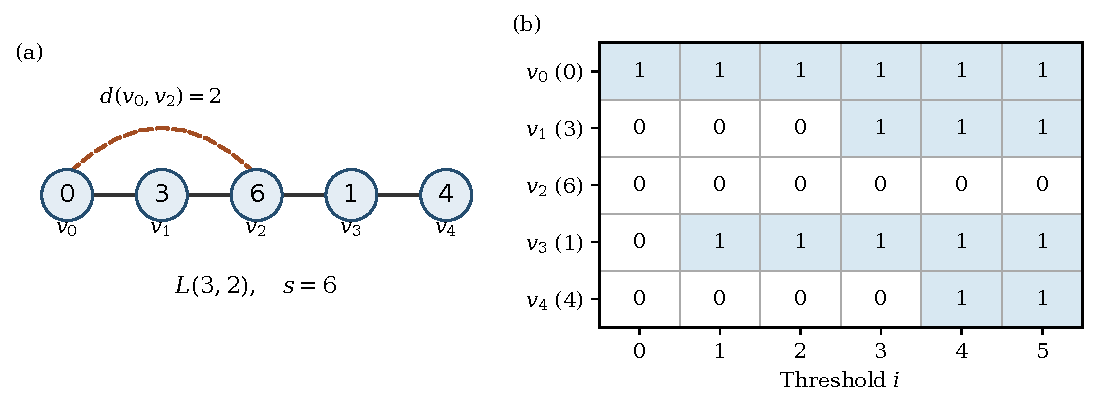
\includegraphics[width=\linewidth]{paper/generated/manuscript_figures/labeling_order.pdf}
\caption{Ví dụ tự dựng: (a) nhãn $0,3,6,1,4$ trên $P_5$ có span 6;
đường nét liền là cạnh, cung nét đứt minh họa một cặp khoảng cách 2, không
phải cạnh mới. (b) Với $s=6$, mỗi ô là $x_{v,i}=[f(v)\leq i]$;
$0\leq i<6$, còn $x_{v,6}=\top$ là hằng. Nhãn đã được validator kiểm tra.}
\label{fig:labeling-order}
\end{figure}
